\section{Dokumentacja techniczna}
\subsection{Hardware}
\label{subsec:hardware}
\subsubsection{Ogólne parametry robota:}
Wymiary zewnętrzne: 180mm x  134mm x 84mm

Masa: 0,5 Kg

Pozostałe najważeniejsze wymiary przedstawiono na Rys.\ref{fig:wymiary}.
\begin{figure}[H]
    \centering
    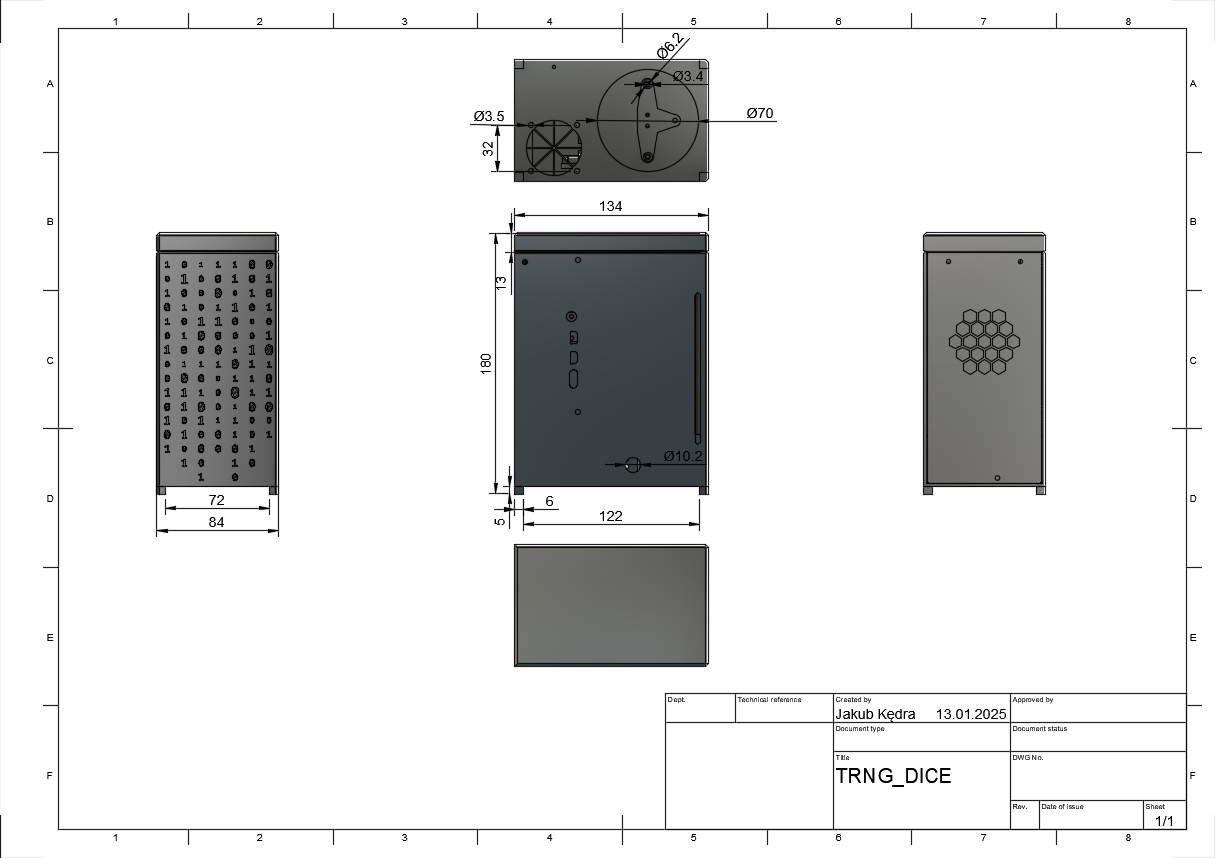
\includegraphics[width=0.95\linewidth]{chapters/03-praca-wlasna/figures/wymiary.png}
    \caption{\label{fig:wymiary}Wymiary zewnętrzne.}
\end{figure}
\textcolor{red}{TODO jak załączyć model 3d}

\subsubsection{Elektronika}
    \begin{itemize}
        \item Raspberry Pi 4B - Komputer wyposażony w czterordzeniowy procesor ARM Cortex-72. Posiada on możliwość łączenia Wi-Fi 802.11ac oraz Bluetooth 5.0. \cite{malina}
        \item Raspberry Pi Camera V2 - Kamera przystosowana do łączenia z Raspberry Pi za pomocą taśmy Raspberry Pi. Posiada ona 8-megapixelowy sensor Sony IMX219. \cite{malina}
        \item L298N - Układ zaprojektowany do przyjmowania standardowych sygnałów TTL wykorzystywany jako sterownik silników.\cite{L298}.
        \item ULN2803A - Układ ten zawiera osiem tranzystorów Darlingtona. Posiada on wspólne emitery oraz wbudowane diody tłumiące dla obciążeń indukcjyjnych.\cite{ULN2803a},
        \item silnik N20 DC 12V z metalową przekładnią 2000RPM.
        \item trzy diody LED 3mm białe.
        \item trzy diody LED 3mm czerwona, niebieska, zielona.
        \item przycisk monostabliny THT.
        \item gniazdo wtykowe DC w formacie 5,5 x 2,1 mm.
    \end{itemize}

\subsubsection{Elementy strukturalne:}
Wszystkie elementy strukturalne wymienione poniżej są zaznaczone na Rys.\ref{fig:komponenty}. Zostały one wydrukowane w technologii FDM na drukarce 3D. Jako materiał do druku części wybrano
PLA \textit{(Polylactic Acid)}. Wyboru dokonano po porównaniu właściwości fizycznych, cen i łatwości wydruku różnych materiałów. Wzięto pod uwagę
PLA, PETG \textit{(Polyethylene Terephthalate Glycol-modified)} oraz ABS \textit{(Acrylonitrile Butadiene Styrene)}. Ostatecznie wybrano PLA, ze względu na jego sztywność, dużą popularność,
niską cenę oraz prostotę procesu druku. ABS odrzucono ze względu na szkodliwe opary podczas druku i potrzebę zamkniętej komory drukarki. PETG najprawdopodobniej
byłby również odpowiednim materiałem do wydrukowania potrzebnych w tym projekcje części, jednak jest on podatny na nitkowanie w czasie druku. Ta cecha
obniżała by jakość wydruku komponentów robota, które zawierają wiele otworów drukowanych w płaszczyźnie pionowej a to sprzyjałoby nitkowaniu. \cite{PLA} \cite{PETG} \cite{ABS} \cite{PLA2}
    \begin{itemize}
        \item obudowa,
        \item tylna ściana obudowy,
        \item górna pokrywa,
        \item kubek,
        \item płytka do montażu kamery i diod LED,
        \item uchwyt do silnika,
        \item płytka do montażu elektroniki,
        \item mocowanie przycisku,
        \item mocowanie sterownika L298,
        \item belka,
        \item śmigło,
        \item nóżki.
    \end{itemize}\
    \begin{figure}[H]
        \centering
        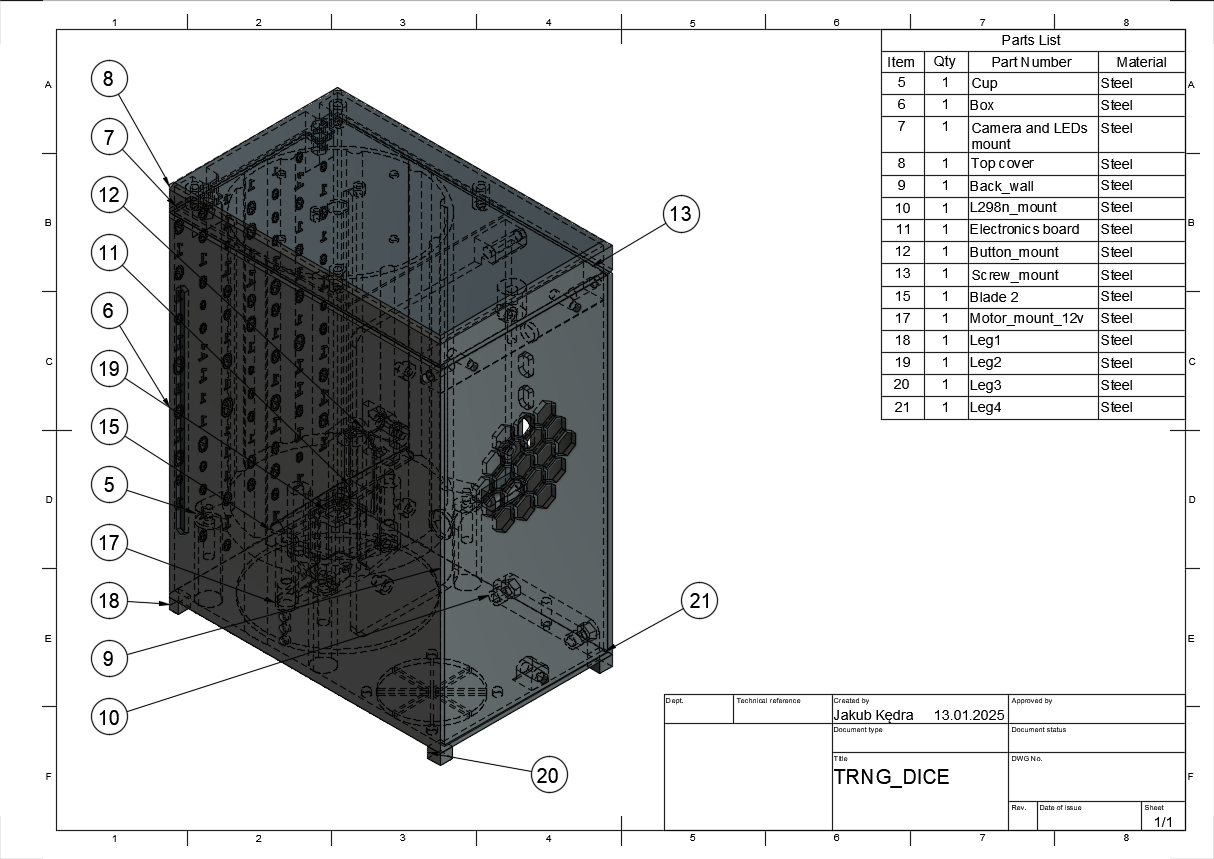
\includegraphics[width=0.95\linewidth]{chapters/03-praca-wlasna/figures/komponenty.png}
        \caption{\label{fig:komponenty}Komponenty robota}
    \end{figure}

\subsubsection{Zasilanie:}
\begin{itemize}
    \item Zasilacz DC 12V - wejście Power Jack 5,5 x 2,1 mm. Wykorzystano zasilacz o mocy 60W, jednak w zupełności do zasilania robota wystarczyłby zasilacz o mocy \textcolor{red}{TODO obliczyć moc i zamieścić tu}
\end{itemize}

\subsubsection{Podłączenie elektroniki}

Schemat na Rys. \ref{fig:electronics} przedstawia wszystkie elementy układu eletronicznego wrac z połączeniami, które zostały wykorzystane w robocie.
Złącza GPIO mikrokontrolera Raspberry Pi 4b zostały użyte do kontrolowania poszczególnych elementów, takich jak silnik prądu stałego oraz diody LED, które są sterowane za 
pośrednictwem układów L298N oraz ULN2803A. Raspberry Pi jest zasilane przez port USB-C, a wszystkie podzespoły dzielą wspólną masę.
Silnik prądu stałego (oznaczony jako M1) jest sterowany za pomocą układu L298N, który umożliwia kontrolę prędkości z jaką obraca się silnik, poprzez kontrolę współczynnika wypełnienia \textit{(Duty cycle)} 
za pomocą sygnału PWM generowanego przez Raspbery Pi i dostarczanego na pin ENB poprzez złącze GPIO. Układ L298N pozwala również na kontrolę kierunku, w którą obraca się silnik poprzez
odpowiednie ustawienie stanów wysokiego i niskiego na pinach IN3 oraz IN4.
Zewnętrzny zasilacz dostarcza napięcie 12V, które zasila zarówno silnik, jak i oba sterowniki - L298N oraz ULN2803A.
Do podłączenia zestawu trzech diod LED (czerwonej, niebieskiej oraz zielonej umieszczonych w gotowym robocie w ściance obudowy robota), wykorzystano rezystory ograniczające napięcie, które podłączono 
do anod poszczególnych diod. Wartości rezystancji dobrano na podstawie zalecanych wartości napięcia dla tych diod oraz w taki sposób żeby ich światło nie było zbyt jasne, ponieważ 
mają to być diody służące tylko do sygnalizowania procesów wykonywanych przez robota. Z tego powodu rezystory, które wybrano mają wyższe wartości rezystancji niż te, które są zalecane, jednak było to
działanie celowe. Dla diod zielonej i niebieskiej wybrano rezystor $10k\Omega$ dla każdej osobno, natomiast dla czerwonej $2,2k\Omega$. Piny GPIO Raspberry Pi odpowiadają za kontrolę włączania poszczególnych diod poprzez sterowanie układem ULN2803A.
Białe diody LED są połączone szeregowo i sterowane za pomocą tranzystorowego układu ULN2803A. W układzie zastosowano rezystory ograniczające napięcie. Każda z tych diod powinna być 
zasilana napięciem od 3V do 3,2V, co oznacza, że po połączeniu szeregowym ich układ powinien być zasilany napięciem 12V, które dostarcza im układ ULN2803A. Zdecydowano się na zastosowanie
rezystorów ograniczających napięcie ze względu na zbyt dużą jasność świecenia tyh diod, co powodowało powstawanie odblasków na kości. Wartości rezystancji tych rezystorów dobrano eksperymentalnie o czym jest mowa w punkcie
i ostatecznie wybrano dwa rezystory połączone szeregowo o rezystancji $2,2k\Omega$ dające łącznie $4,4k\Omega$. \textcolor{red}{TODO sprawdzic te wartości bo cos mi nie pasuje}
Dodatkowo układ zawiera mały wentylator (Fan1), zasilany napięciem 12V. W rzeczywistości w robocie wykorzystano szynę zasilania, z której zasilane są wszystkie wspominane komponenty. 
Schemat zawiera także przycisk (S1), który jest wykorzystywany jako prosty przełącznik do wywołania sygnału wejściowego na jednym z pinów GPIO Raspberry Pi.

\begin{figure}[H]
    \centering
    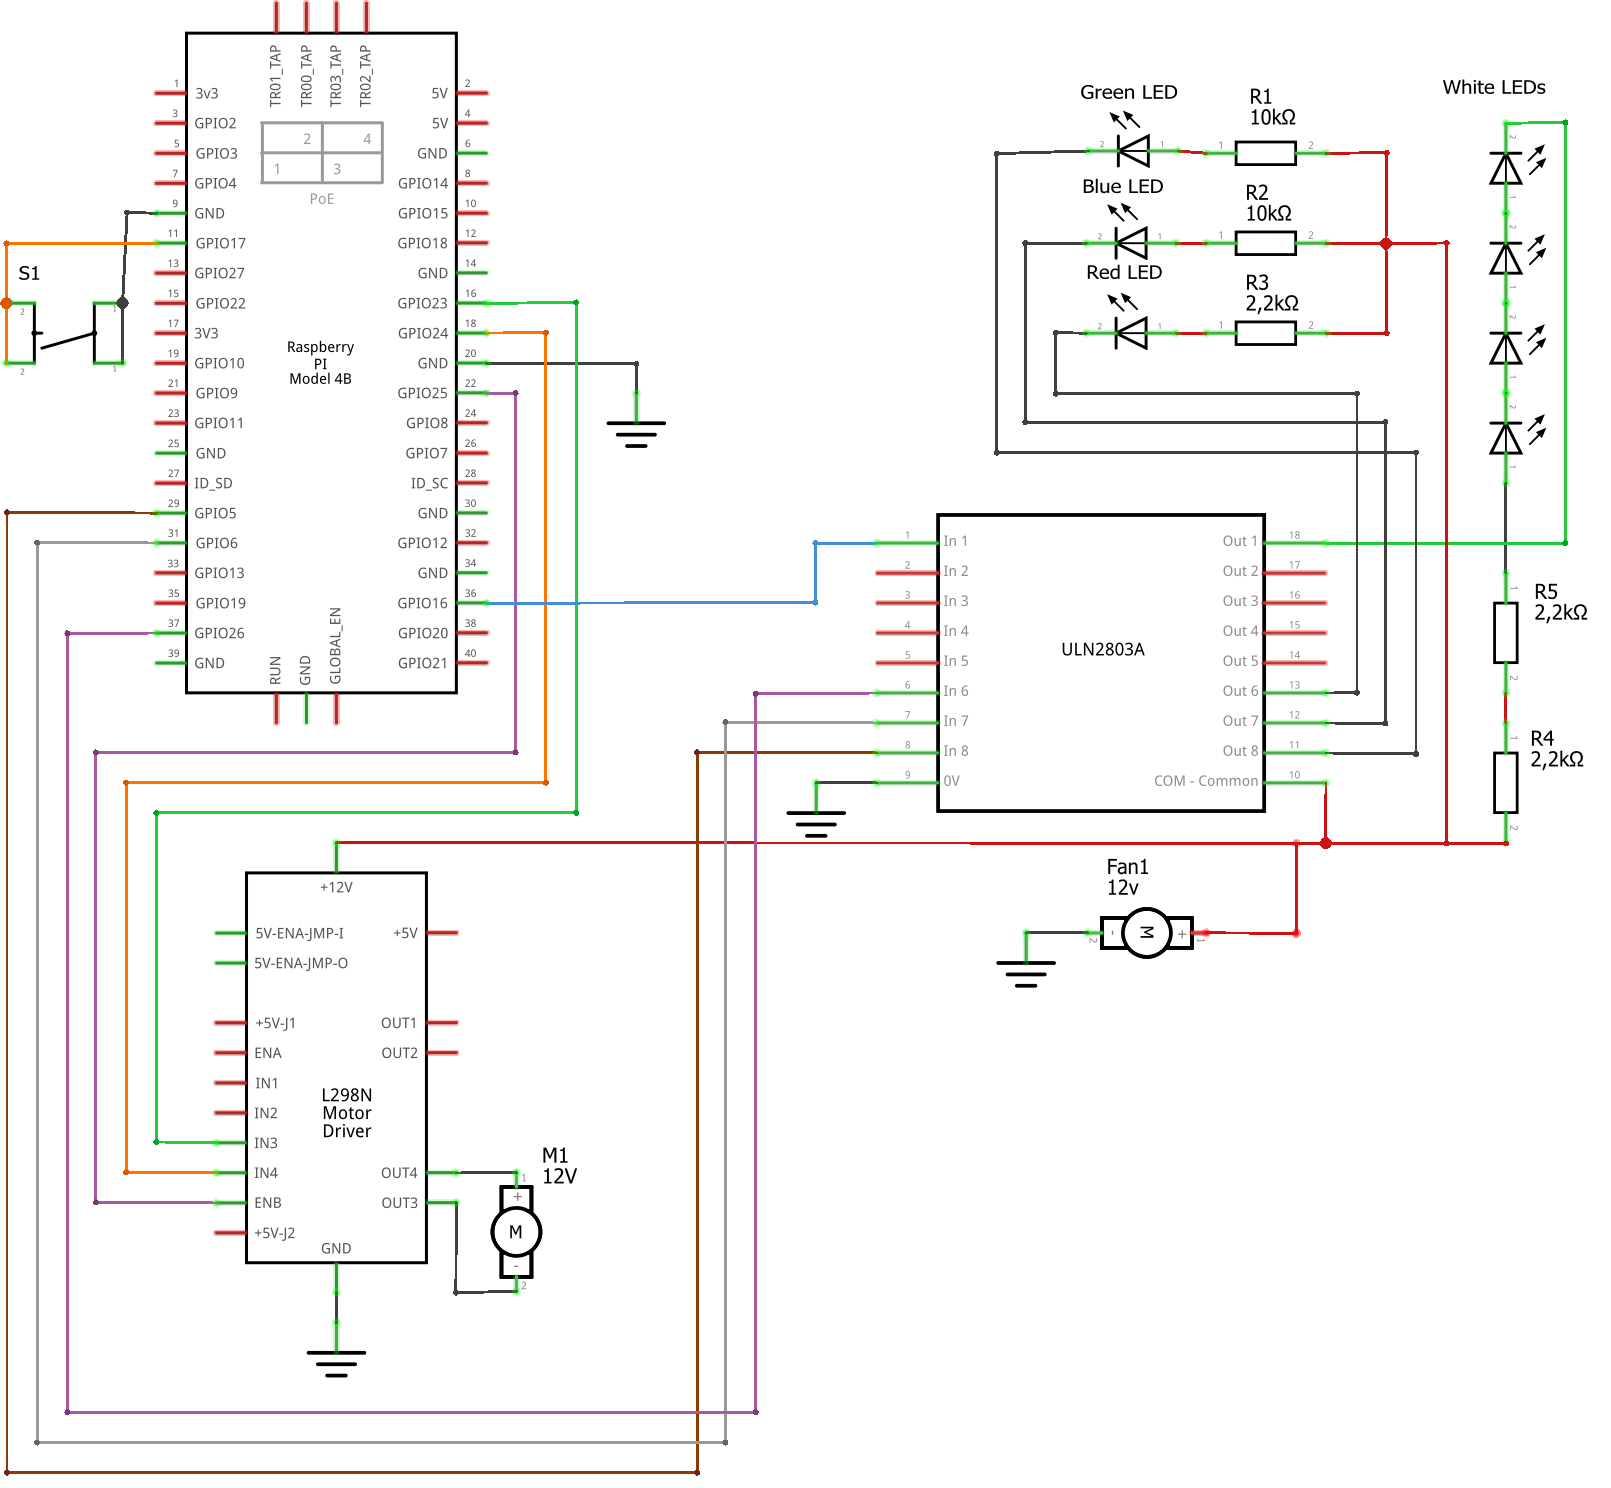
\includegraphics[width=0.95\linewidth]{chapters/03-praca-wlasna/figures/electronics circut_schem.png}
    \caption{\label{fig:electronics}Schemat elektryczny.}
\end{figure}

\subsection{Software}
bbbbbbbbbbbbbbbbbbbbb